\documentclass[../main.tex]{subfiles}

\begin{document}
    
\chapter{Optimal Sector Universes} \label{optimal_sector_universes}


In this chapter, we utilize the backtesting system outlined in the previous chapter, we performed historical universe-level analysis of each of our candidate learned sectors. To reiterate, we plan to use the SETF restructuring turnover, the portfolio rebalancing turnover, the portfolio value, and the Sharpe ratio to rank our candidate learned sectors againt each other.

Due to the magnitude of data output by the reIndexer backtesting system, all calculations in this section were performed in the cloud, on Google Research Colaboratory.\citeFormat{\cite{GoogleResearch2019GoogleColaboratory}} Data was loaded dynamically from its output location on Google Drive, directly into Google Colaboratory. Following this, individual output files were opened sequentially to extract the necessary longitudinal data dimension for the candidate learned sector universe, with all data being kept in-memory on Google Cloud Platform servers for increased efficiency during analysis.\citeFormat{\cite{Weerawarana2019LearnedAnalytics}}

\section{Complete Backtest Results}

The complete results of the backtest are published online, and are available on the reIndexer website.\citeFormat{\cite{Weerawarana2019ReIndexerUniverses}}

Due to the magnitude of data generated by reIndexer, it is impractical to display quantitative summaries for each sector. Rather, we plotted graphs to visualize the progression of each of the risk metrics discussed in Section~\ref{candidate_universe_ranking:eval_metrics}. The graphs were plotted for the full backtesting window outlined in Section~\ref{candidate_universe_ranking:backtest_config}.

\begin{itemize}
    \item Cumulative SETF Restructuring Turnover (Figure~\ref{fig:appendix_backtest:setf_restructuring_turnover})
    \item Cumulative Portfolio Rebalancing Turnover (Figure~\ref{fig:appendix_backtest:portfolio_rebal_turnover})
    \item Portfolio Value (Figure~\ref{fig:appendix_backtest:portfolio_return})
    \item Rolling Sharpe Ratio (Figure~\ref{fig:appendix_backtest:sharpe_ratio})
\end{itemize}

See Appendix~\ref{appendix:backtest_visualization} on Page~\pageref{appendix:backtest_visualization} for full-sized plots of each of the graphs.

% \pagebreak

\section{Backtest Results Analysis}

We computed and recorded each of the Performance Evaluation Metrics outlined in Section~\ref{candidate_universe_ranking:eval_metrics} for each time step across all 60 candidate learned sector universes.

Following this, we computationally extract the optimally performing learned sector universe for each of the performance metrics. As both turnover metrics track a cost, we isolated the learned sector universe with the minimum cumulative value at the end of the simulation. Conversely, we isolated the learned sector universe that yielded the maximimum value for both the portfolio value, and the (average) rolling Sharpe ratio.

We now discuss the optimally peforming learned sector universe with respect to the turnover and maximum absolute portfolio value metrics. Coincidentally, the minimum cumulative SETF restructuring turnover, and the minimum portfolio rebalancing turnover are both achieved by the same learned sector universe. These two performance metrics will be discussed together.

\subsection{Minimum Cumulative Turnover}

\begin{wrapfigure}[22]{r}{0.5\textwidth}
    \centering
    \vspace{\wrapfigadjustment}
    \fbox{
    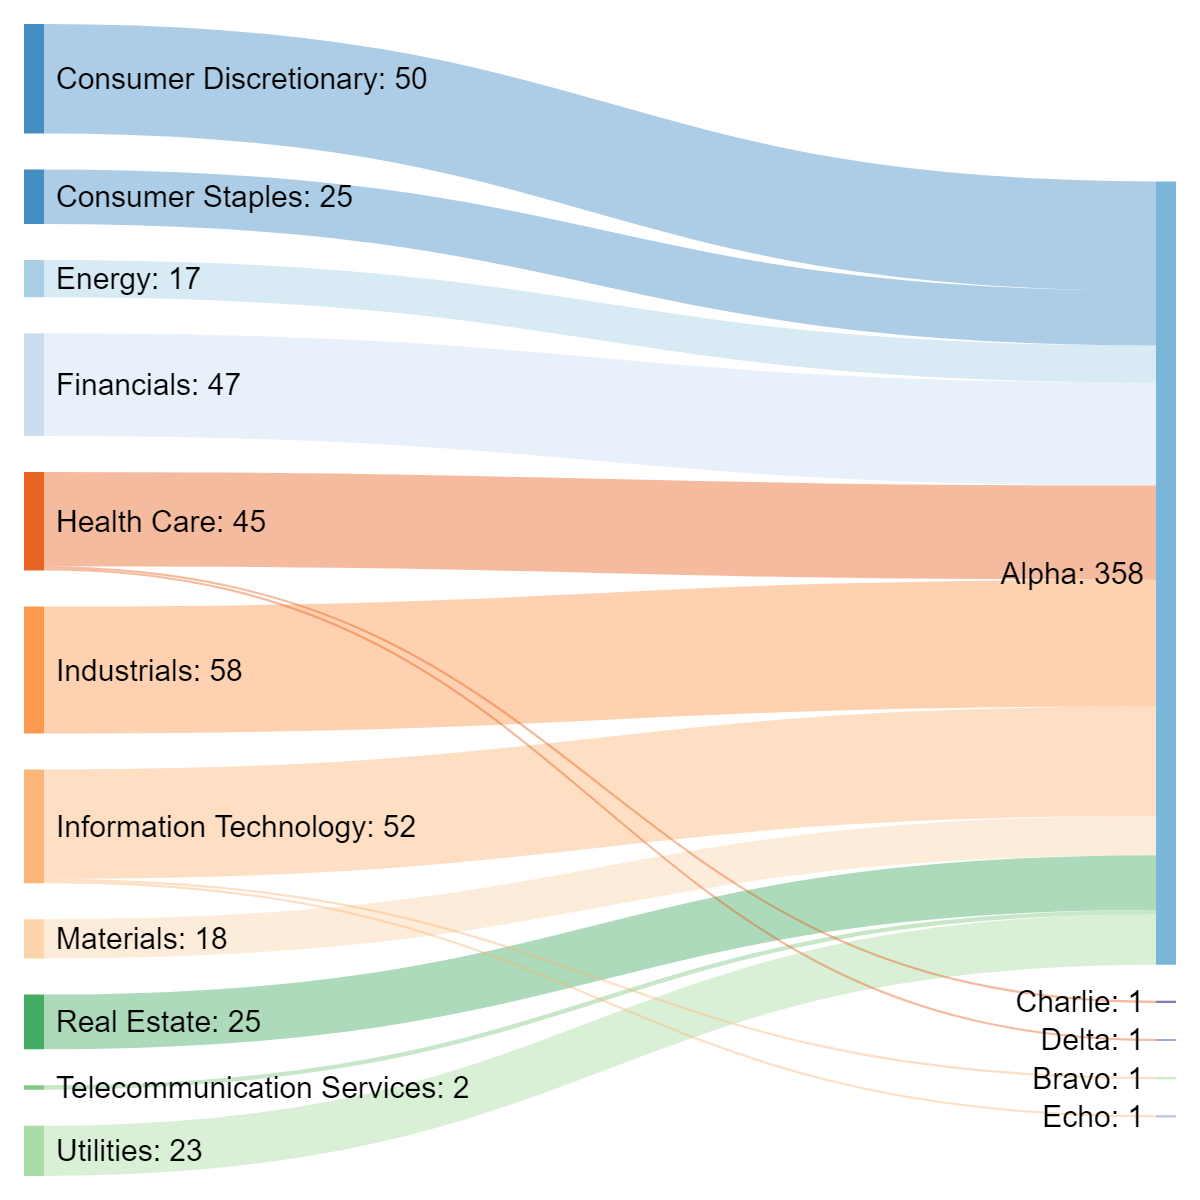
\includegraphics[width=.9\linewidth]{images/single_2017_5.png}
    }
    \caption{Learned sector universe with minimum cumulative SETF restructuring, and portfolio reblancing turnover.}
    \label{fig:optimal_sector_universe:minimum_turnover}
\end{wrapfigure}

As discussed in Section~\ref{candidate_universe_ranking:eval_metrics}, the cumulative turnover, for both SETF restructuring, and portfolio rebalancing, are designed to be a proxy for the cost of issuing, and holding these ETFs, respectively. The learned sector that performed best with respect to the cumulative turnover metrics has the following configuration:

\vspace{0.5em}

\begin{minipage}{\linewidth}
    \centering
    \bfseries
    \fbox{
        Single Linkage; 5 Sectors
    }
\end{minipage}

\vspace{0.5em}

The cost proxies each measure the effective cost of the SETF for entirely different segments of the Financial Lifecycle of this hypothetical product. The SETF restructuring turnover is a proxy for the cost that would be incurred by an ETF issuer (i.e. an institutional investor), whereas the portfolio rebalancing turnover is a proxy for the cost incurred by a holder of the ETF (i.e. a retail investor).

Upon closer inspection of the Sankey diagram corresponding to this sector in Figure~\ref{fig:optimal_sector_universe:minimum_turnover}, it is clear why it has superior minimum turnover, through the lens of both SETF restructuring, and portfolio rebalancing. The presence of a single large sector containing most of the assets (all of the assets with the exception of 4 in the case of Figure~\ref{fig:optimal_sector_universe:minimum_turnover}) implies that the sector universe would inherently have a significant advantage over its counterparts.

This single-sector pooling behavior would imply its SETF restructuring fee would be 0 in perpetuity for the sectors in which there is only a single asset. As single-asset sectors represent 80\% of the sectors in this universe, this result is not surprising. This advantage is conferred in a similar fashion to the portfolio restructuring fee, as single-asset sector SETFs are not likely to be held in large quantities, relative to the singular vast sector SETF (Sector \textit{Alpha}, in this example).

Unfortunately, it seems that the single linkage method results in a significant \textit{pooling} effect, where the vast majority of assets are relegated to a single sector, with the remaining sectors being relative extremely small; containing just one asset each in the case of Figure~\ref{fig:optimal_sector_universe:minimum_turnover}. This behavior under the single linkage method is apparent from both the underlying data, as well as the partial search space visualization in Figure~\ref{fig:hierarchical_clustering_model:partial_search_space}.

% \pagebreak

\subsection{Maximum Absolute Portfolio Value}

\begin{wrapfigure}[23]{L}{0.5\textwidth}
    \centering
    \fbox{
    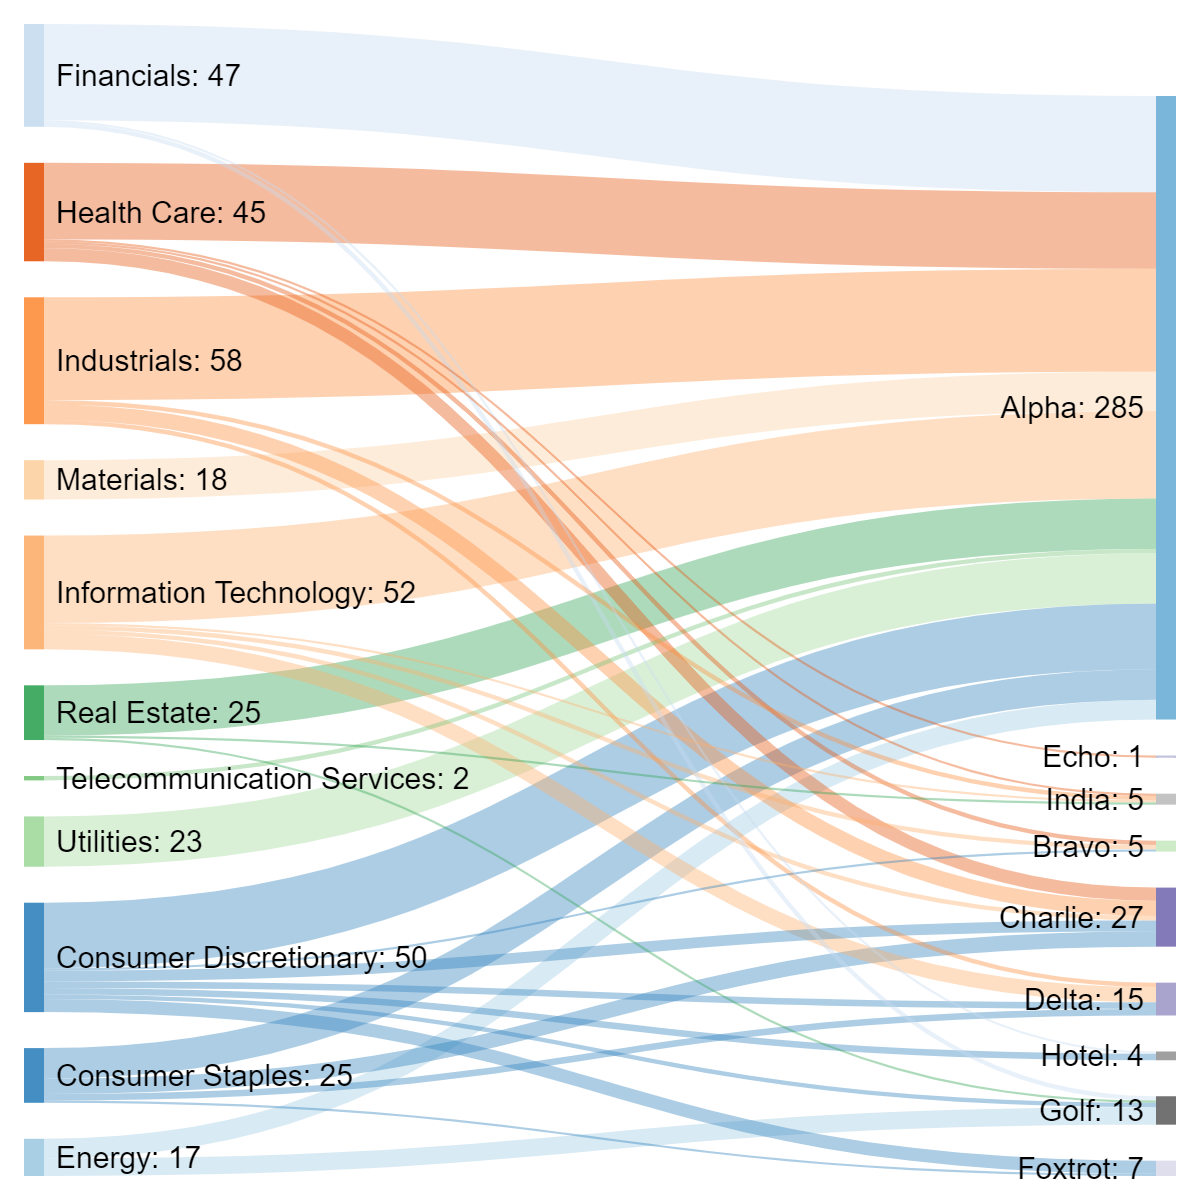
\includegraphics[width=.9\linewidth]{images/complete_2017_9.png}
    }
    \caption{Learned sector universe with maximum absolute portfolio value.}
    \label{fig:optimal_sector_universe:max_return}
\end{wrapfigure}

Unlike the previous performance metric, evaluating the historical learned sector universe portfolio value is not a proxy for an external cost. Rather, it is a candid assessment of the historical performance of the learned sector universes. While this does not directly address any of our research goals, it is an extremely important performance metric, and would be a key determinant of the success of any given learned sector universe in the real market. The learned sector that had the maximum absolute portfolio value over the lookback period (outlined in Section~\ref{candidate_universe_ranking:backtest_config}) has the following configuration:

\vspace{.5em}

\begin{minipage}{\linewidth}
    \centering
    \bfseries
    \fbox{
        Complete Linkage; 9 Sectors
    }
\end{minipage}

\vspace{.5em}

The absolute portfolio value tracks the value of the portfolio throughout the backtesting period, utilizing the nested value computation outlined in Section~\ref{candidate_universe_ranking:port_optim}. While not being a direct proxy of risk diversification, if viewed through the lens of potentially improved economic asset grouping, this learned sector universe is extremely encouraging. If the corollary that better capital market performance is correlated with improved economic sector performance, this result would imply that the fundamentals-driven classification heuristic does indeed provide a beneficial measure of diversification.

Unlike the previous learned sector universe under the Single Linkage Method, the learned sector outlined in Figure~\ref{fig:optimal_sector_universe:max_return} appears to have significantly less pooling. Despite this however, assets are still highly concentrared in a single extremely large sector, with other sector sizes (with respect to the number of constitutent companies) being significantly smaller.

An interesting observation of this sector is that there is significant dispersion from the original benchmark classification. Omitting the sector \textit{Alpha} due to its gargantuan size, sectors \textit{Charlie} and \textit{Delta} both have numerous components from highly diverse original benchmark sectors. Sector \textit{Charlie} appears to have a high number of assets from the \textit{Health Care} sector, as well as the \textit{Industrials} and \textit{Consumer Discretionary} sectors. Similarly, sector \textit{Delta} has a large number of constiutent assets classified as \textit{Information Technology}, \textit{Consumer Staples}, and \textit{Consumer Discretionary} under the benchmark classification.

As with the sample sector classification discussed in Section~\ref{candidate_universe_ranking:sample_ls}, there appears to be high levels of dispersion of assets in sectors which are increasingly requisite to doing business. This is particularly evident (again, ignoring sector \textit{Alpha}) through the dispersion of the \textit{Information Technology}, \textit{Health Care}, and \textit{Consumer Discretionary} sectors.


\section{Risk-Adjusted Return Optimal Universe} \label{optimal_sector_universe:risk_adj_return_optimal}

Finally, to isolate the sector with the maximum rolling annualized Sharpe ratio, we computed the mean rolling Sharpe ratio across the longitudinal temporal axis, and compared each of the learned sectors. Following this comparison, we determined that the learned sector that had the maximum average rolling Sharpe Ratio over the lookback period has the following configuration:

\begin{minipage}{\linewidth}
    \centering
    \bfseries
    \fbox{
        Complete Linkage; 17 Sectors
    }
\end{minipage}

\vspace{1em}

The Sankey diagram corresponding to the risk-adjusted return optimal learned sector is displayed in Figure~\ref{fig:optimal_sector_universe:max_sharpe}. As indicated by the diagram, this learned sector universe has even less pooling behavior that both of the previously discussed learned sector universes (Figure~\ref{fig:optimal_sector_universe:minimum_turnover} and Figure~\ref{fig:optimal_sector_universe:max_return}), despite still having 2 relatively large sectors, \textit{Alpha}, and \textit{Golf}, when compared to the rest.

As this learned sector universe provides the best risk-adjusted return on an already variance-minimized Global Minimum Variance Portfolio comparison, it would imply that this configuration provides the best risk diversification profile out of all of the candidate learned sector universes. In addition to the obviously highly prevalent dispersion from the benchmark classification to the new learned sectors, the size of each of the sectors is also consierably more even compared to its peers. This would imply a better portfolio-level diversification profile, as poorly performing sectors can be underweight during times of low implied risk-adjusted return. This is a key caveat of the pooling behavior particularly prevelant under the Single Linkage heuristic.

\begin{figure}[h]
    \centering
    \fbox{
        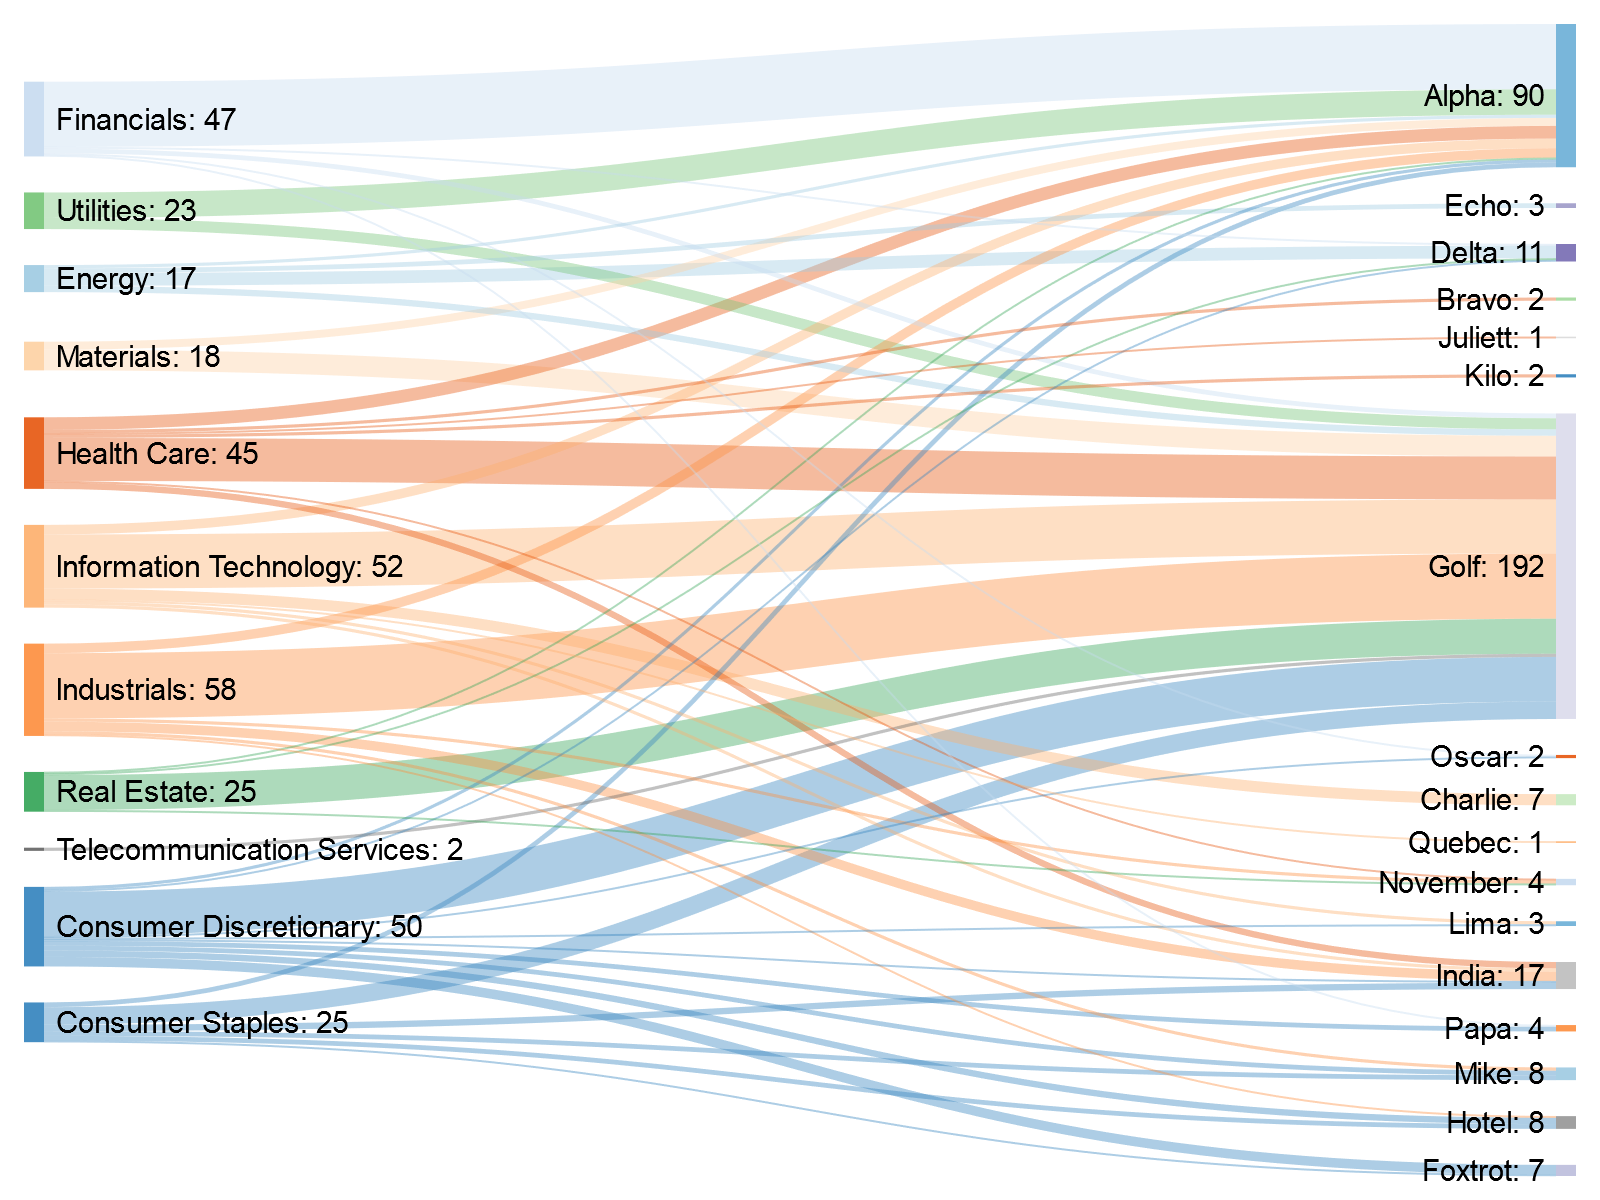
\includegraphics[width=0.9\linewidth]{images/complete_2017_17.png}
    }
    \caption{Learned sector universe with maximum rolling Sharpe ratio.}
    \label{fig:optimal_sector_universe:max_sharpe}
\end{figure}

This lack of transitivity, combined with the implication that a higher risk-adjusted return implies a better risk-diversification profile would suggest that the learned sector universe heuristic is providing high levels of economic diversification, which appears to be at odds with the benchmark classification.

\end{document}